%%%%%%%%%%%%%%%%%%%%%%%%%%%%%%%%%%%%%%%%%%%%%
\subsection{Extracting \scc{s}}
\label{sec:log-analysis}
%%%%%%%%%%%%%%%%%%%%%%%%%%%%%%%%%%%%%%%%%%%%%

%% \item Construct a lattice structure which models all cuts of the log
%%   such that the happened-before relation is respected in each cut.

%% \item Enumerate sent and received messages for each node in the log,
%%   and reduce the lattice to cuts with no outstanding messages, the
%%   reduced lattice is the set of all consistent cuts.

%% Inferring valid distributed data invariants is a multi-faceted
%% problem. The majority of the challenges arise from concurrency. Nodes
%% which undergo concurrent state changes may simultaneously reach a
%% state which falsifies an invariant property, only to return to a state
%% in which the invariant is satisfied upon communicating again. In such
%% cases the invariant is falsified, but without a mechanism for
%% reasoning about partial ordering the property cannot be checked. The
%% following is a list of challenges inherent to checking distributed
%% invariants which our techniques address.

%% \begin{enumerate}
%% %
%%     \item The number of partially ordered \emph{events} are
%%         exponential in the number of nodes. In order to reason about
%%         the full set of partial orderings a complete model of this
%%         space must be constructed.
%% %
%%     \item Distributed state is not always resident on the nodes of the
%%         system. Analysis on distributed state is incomplete if any
%%         state is in transit.
%% %
%%     \item Distributed systems are highly variable in their both their
%%         communication patters, topologies, and node hierarchies.
%%         Determining the granularity at which to test for distributed
%%         invariants is therefore system, and property dependent.
%% %
%% \end{enumerate}
%

%% Without using any mechanism for reasoning about the order of
%% \emph{event}s in a distributed system, the number of possible
%% \emph{event} orderings is exponential. Testing invariant properties on
%% every interleaving combination of events would not only be extremely
%% costly, but also produce invariants inconsistent with the systems
%% execution. Vector clocks establish a partial ordering on events
%% between communicating nodes. However, the growth of partial orderings
%% is still exponential on events which occur between
%% communication.

%%%%%%%%%%%%%%%%%%%%%%%%%%%%%%%%%%%%%%%%
\begin{figure}[t]
    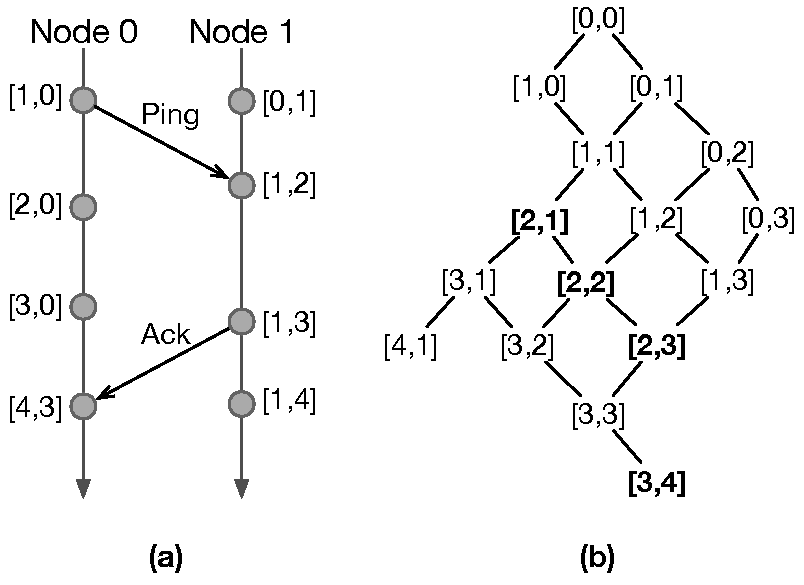
\includegraphics[width=0.50\textwidth]{fig/time-diagram}
    \caption{\textbf{(a)} Space-time diagram of an execution of code
      in Figure~\ref{fig:data-flow} with two nodes, Node 0 and Node
      1. \textbf{(b)} Lattice corresponding to this execution with
      \scc{s} indicated in bold.}
\label{fig:time-lattice} 
\end{figure}
%%%%%%%%%%%%%%%%%%%%%%%%%%%%%%%%%%%%%%%%

%% Figure~\ref{fig:time-lattice} shows a send from $H1$ at time
%% $C_{H1}[H1] = 1$ and a receive on $H2$ at time $C_{H2}[H1]=1,[H2]=2$
%% This event constrains possible event orderings.  More precisely it is
%% established that all events $C_{H1}[H1] <= 1$ happened before
%% $C_{H2}[H2] >= 2$. Therefore all ordering $C_{H2}[H2] < 2$ ,
%% $C_{H1}[H1] > 1 $ are invalid.  Such values are not part of the
%% lattice.  More formally $\forall Host_i,$ such that $Host_i$ logged a
%% clock value $C[i] = t$ all lattice clocks with value $C[i] = t$
%% Happened after the logged node event instance.

A lattice contains all event orderings consistent with the
happens-before relation~\cite{Cooper:1991:CDG:122759.122774}. This
property constrains the exponential set of potential event orderings
and supplies a complete view of a systems execution. A variety of
different algorithms for constructing a lattice have been
proposed~\cite{Garg}. Appendix~\ref{sec:lattice-appendix} presents our
algorithm for constructing the lattice.

Figure~\ref{fig:time-lattice} shows the time-space diagram and
corresponding lattice for an execution of two nodes, Node 0 and Node 1,
each of which runs the code in
Figure~\ref{fig:data-flow}. Node 0 sends a \emph{ping}, executes
two local events, then receives an \emph{ack} message.

%
% JS: scc expands to strongly consistent cut. articles missing.
%     sometimes it should be pluralized. the set of \scc{}_s_.
%
Within this lattice, \scc can be computed by enumerating sent and
received messages. We use the set of \scc in the lattice as our
granularity for inferring invariants (highlighted in bold in
Figure~\ref{fig:time-lattice}B). Merging the states of interacting
nodes at the granularity of \scc guarantees that the sum of node
states is representative of the state of the system.
Algorithm~\ref{alg:mineCuts} shows our process for extracting
consistent cuts from a lattice.

%% A variety of algorithms exist for computing consistent cuts from the
%% execution of a distributed system~\cite{MATTERN1993423}. A high level
%% description of our algorithm is given here, a full overview is given
%% in Section~\ref{sec:consistent-cuts-appendix}. We process the log by
%% enumerating sent and received messages and maintaining a delta for
%% each node. Points in the lattice on which the sum of each nodes delta
%% equals zero are to consistent cuts. This calculation is run on every
%% point in the lattice, the result is a complete set of consistent cuts.
%% Finally the states of nodes at the logical time corresponding to a
%% consistent cut are collected together. The output of this process is
%% the complete set of node states at every point during execution when
%% all state was resident in memory.

%% Figure~\ref{fig:time-lattice}B shows a lattice
%% structure of all possible partial orderings of events which respect
%% the happens-before relationship established by vector clocks.
%% We use the lattice of partial orderings as a model for accurately
%% describing a distributed execution. Algorithm~\ref{alg:lattice} is a
%% high level overview of our lattice construction algorithm.

%% Using a lattice to model distributed execution provides a complete
%% view of the execution. However, not every point on the lattice
%% is appropriate for testing invariants. Distributed state has
%% two possible locations, either resident on a node, or in
%% transit on a wire. In the latter case the state of the system
%% is unobservable.  Lattice points at which state is in
%% transmission provide only a partial view of distributed
%% state. Testing invariants at such points would be incorrect as
%% state which could falsify a property may not be
%% present. \emph{Consistent cuts} of a network are points in
%% relative time at which no messages are in transit.

%% Distributed systems are designed for a variety of purposes.  Their
%% behaviour, communication patterns, and desired invariants are also
%% highly varied. For example leader election algorithms, and
%% peer-to-peer systems typically have multiple nodes running identical
%% code, whereas client-server systems have distinct functionality.
%% Invariant properties hold at differing granularity's subject to the
%% architecture of the system. No one strategy for testing invariants
%% would detect every desired property in arbitrary systems.  Our
%% approach to this problem makes use of 3 heuristics for testing
%% invariants at differing granularity's of the systems execution.

%% In this section we describe the structures and processes we use to
%% collect the set of all consistent cuts from an execution log, merge
%% the logged states of nodes into distributed program points, and test
%% merged states for invariants. The following is a high level overview
%% of our process.

%%%%%%%%%%%%%%%%%%%%%%%%%%%%%%%%%%%
\begin{algorithm}[t]
    \KwData{A system log $L$}
    \KwResult{A set of consistent node states $S$ }
        $clocks$ := vectorClockArraysFromLogs($L$)\\
        $lattice$ := buildLattice($clocks$)\\
        $deltaComm$ := enumerateCommunication($clocks$)\\
        $cuts$ := mineConsistentCuts($lattice$, $clocks$, $deltaComm$)\\
        $S$ := statesFromCuts($cuts$, $clocks$, $logs$)\\
    \Return $S$
    \label{alg:mineStates}
    \vspace{2mm}
    \caption{High level log merging overview}
\end{algorithm}
%%%%%%%%%%%%%%%%%%%%%%%%%%%%%%%%%%%


%%%%%%%%%%%%%%%%%%%%%%%%%%%%%%%%%%%%%%%%%%%%%%%%%%%%%%%%%%%%%%%%%%%%%%%%%%%%%%%%%%%%%%%%
\subsection{Merging cuts into distributed program points}
\label{sec:merging}
%%%%%%%%%%%%%%%%%%%%%%%%%%%%%%%%%%%%%%%%%%%%%%%%%%%%%%%%%%%%%%%%%%%%%%%%%%%%%%%%%%%%%%%%

%% \textbf{Apply a merging strategy to consistent cuts to produce sets of
%%   distributed program points.}

%
% JS: ``their states and variables'', you mean the nodes'?
%     Maybe instead: To check local invariants hold on multiple nodes,
%     we merge variable states.

To check state invariants on multiple nodes, their states are merged
together and their variables are tested for invariants. All logged
states are related to the program points where they were logged.  We
therefore define a merged set of states to be a \emph{distributed
  program point}. Determining which states to merge when checking for
particular invariants is difficult because distributed systems have a
variety of communication topologies. 

For example, nodes in a client-server system execute different code,
while nodes in a distributed hash tables are identical peers whose
behaviour is dictated by their unique identifier. In each case the
system's invariant properties hold at different levels, and require
alternative views of the execution to test them. Checking that all
nodes in an election agree on a result, or that all DHT peers agree on
where to route a request requires a system wide view.  Checking that a
server responds idempotently to client requests only requires a view
between a client and the server. Checking that state updates are
propagated through a gossip protocol requires a view specific to the
dataflow in the system.

%% solutionNo one strategy for extracting distributed invariants will
%% work the desired property in an arbitrary system. Our solution is
Instead of a one-size-fits-all approach we use 3 heuristics for
merging node state for inferring invariants: (1) merge the states of
all nodes in a \scc, (2) merge only the states of unique pairs of
senders and receivers, and (3) merge the states of nodes that
participated in a totally ordered communication.
    
%%%%%%%%%%%%%%%%%%%%%%%%%%%%%%
\begin{figure}[h]
    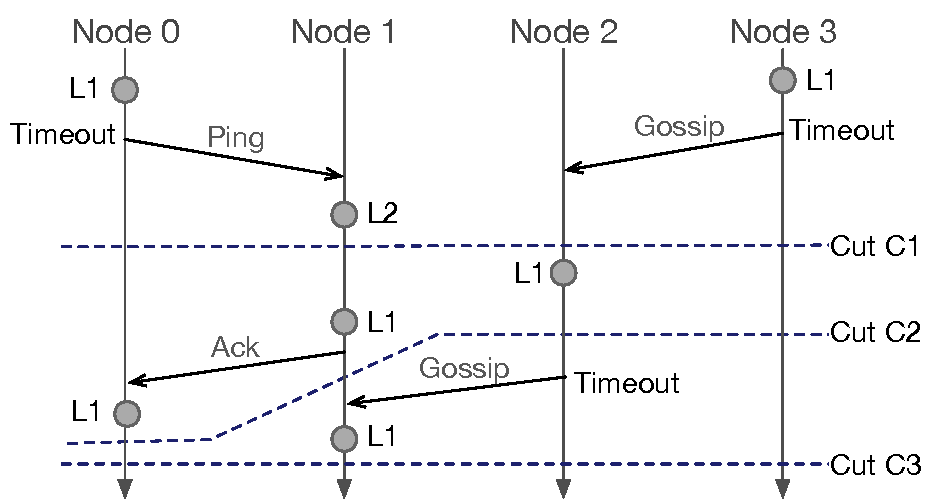
\includegraphics[width=0.5\textwidth]{fig/gossip-execution-dig}
    \caption{Sample SWIM execution with 4 nodes running code from
        Figure~\ref{fig:data-flow}. This diagram is a subset of a
        larger execution. Points $L1$ and $L2$ on each node timeline
        represent the execution of two separate logging functions. $L1$
        and $L2$ corresponds to lines 12 and 6 in
        Figure~\ref{fig:data-flow} respectivly.  Dashed lines $C1$,
        $C2$, $C3$ are \scc{s} of the execution including just these 4
nodes.} \label{fig:gossip-execution} \end{figure}
%%%%%%%%%%%%%%%%%%%%%%%%%%%%%%

%%%%%%%%%%%%%%%%%%%%%%%%%%%%%%
\begin{figure}[h]
%    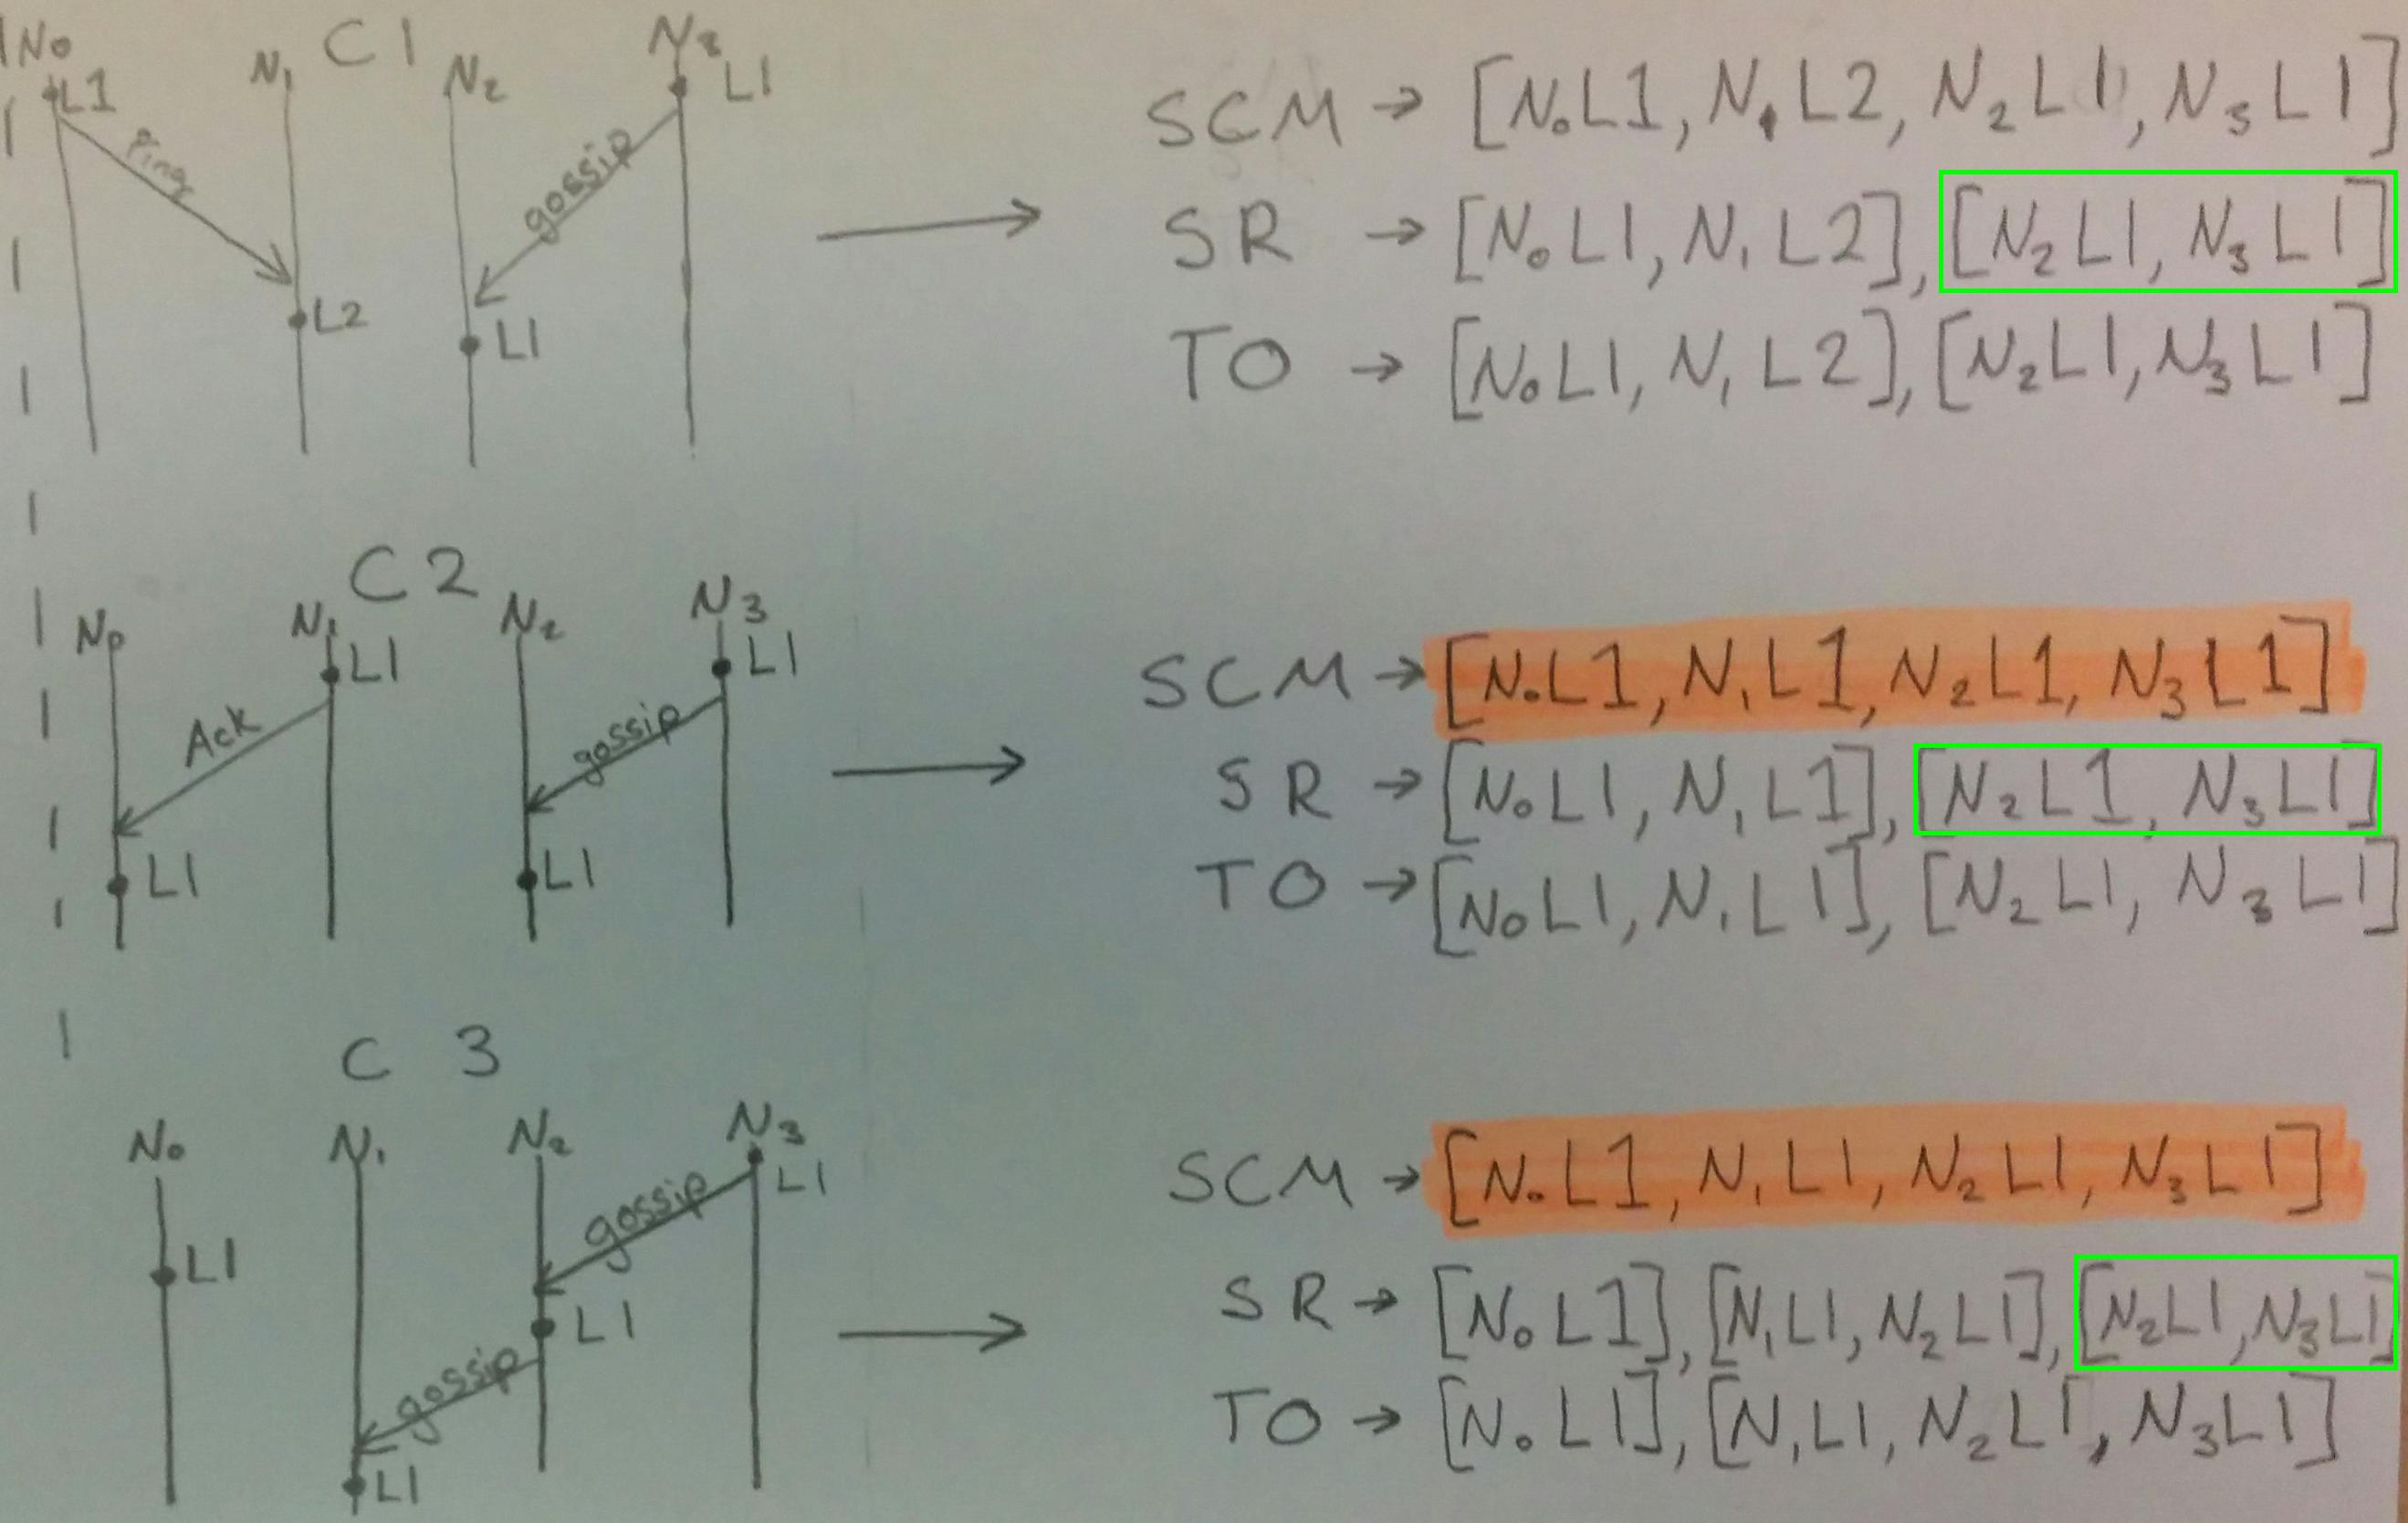
\includegraphics[width=0.5\textwidth]{fig/cuts-to-dpp}
    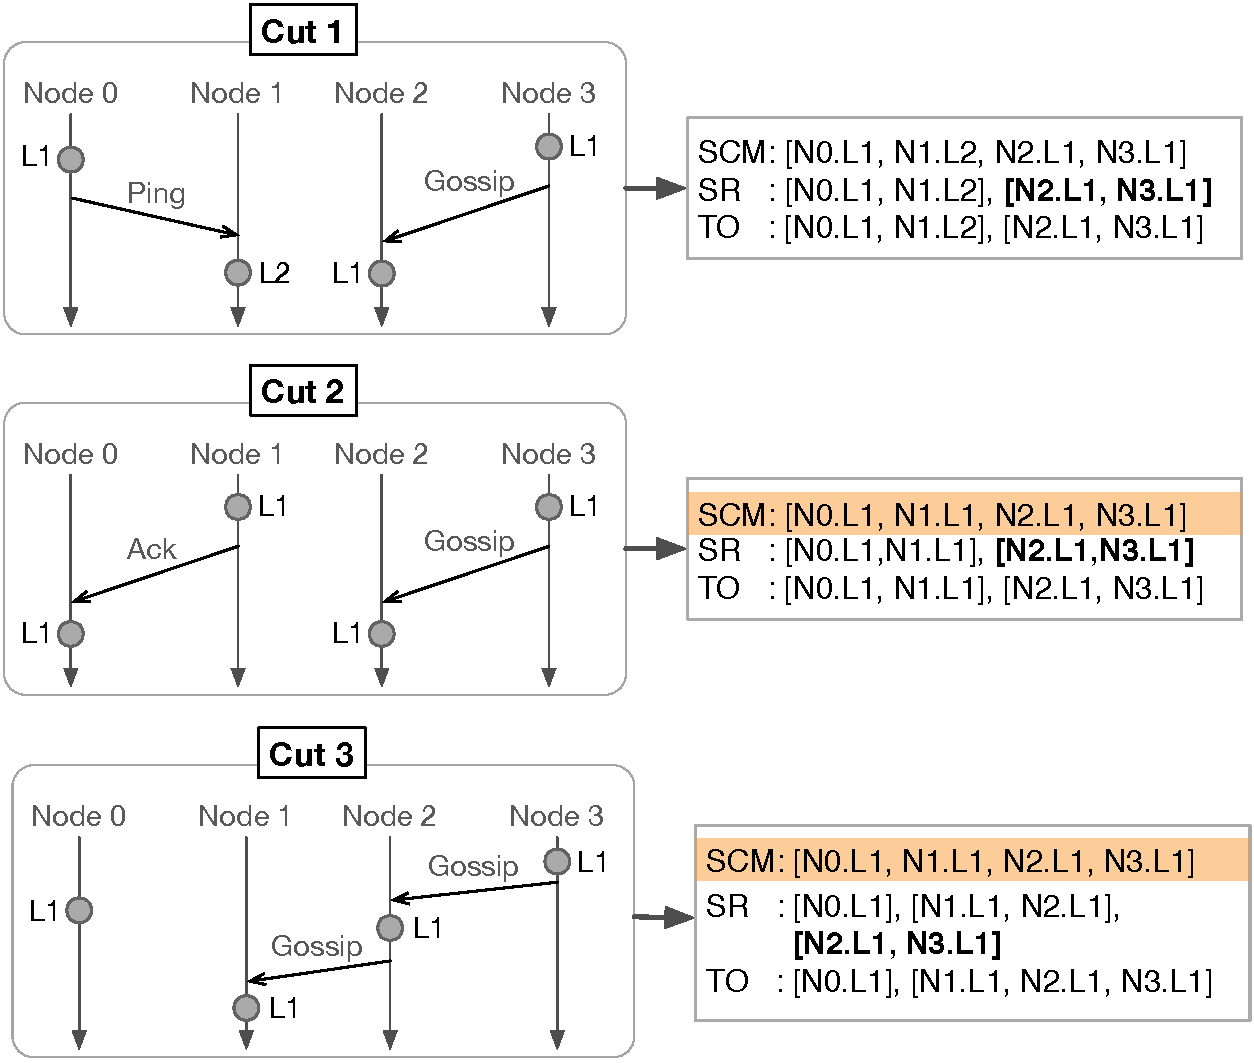
\includegraphics[width=0.5\textwidth]{fig/cuts-to-dpp-dig}
    \caption{Illustration of the three merging strategies that convert
      cuts into sets of distributed program points. On the left, are
      cuts $C1$, $C2$, $C3$ from Figure~\ref{fig:gossip-execution}
      depicted as sets of logged state. The right side shows how the
      three merging strategies, \textbf{WCM}: whole cut merge,
      \textbf{SR}: send-receive merge, and \textbf{TO}: total order
      merge, produce different distributed program points. Highlighted
      are two matching distributed programs points.}
\label{fig:cuts-to-dpp}

\end{figure}
%%%%%%%%%%%%%%%%%%%%%%%%%%%%%%

% JS: watch out for orphans and widows here.
%
\textbf{Whole cut merge.}  This merge is performed by collecting the
states of all hosts in a \scc and testing them for
invariants together.  Invariants which are true for all nodes on all
\scc are checked at this granularity. For example in a
distributed hash table where resources are not duplicated across
multiple nodes an invariant such as $\forall i,j \in nodes$ $i-keys !=
j-keys$ would be detected.  In other cases whole cut merge will not
detect invariant properties.  Figure~\ref{fig:cuts-to-dpp} shows the
whole cut merged points from a Serf execution. Checking Serf's eventual
consistency invariant with whole cut merge would not work. In the
example, if the whole cut merge distributed program point from $C1$ and
$C3$ were checked for invariants, \dinv would detect that $N_0-Events
!= N_3-Events$ because the gossip message from $N_3$ had yet to
propagate to $N_0$. Whole cut merge falsifies Serf's consistency
invariant because at the granularity of a \scc the property
does not hold.

\textbf{Send-receive merge.} In some cases it is necessary to analyze
the states of pairs of interacting nodes. In such cases merging the
states of senders and receivers in a \scc can be used to verify
invariant properties of their isolated interaction.
Figure~\ref{fig:cuts-to-dpp} details how send-receive merge constructs
distributed program points. The state of a sender immediately before a
send is merged with the state of the receiver immediately after
receiving. \textit{Cut C3} details how states are merged in cuts where
nodes both sent and received messages, as well as nodes which did not
communicate. In the case of no communication the node state is left
isolated. Whole cut merge fails to detect eventual consistency, but
the invariant can be verified with send-receive merge. In the case of
Figure~\ref{fig:cuts-to-dpp} inferring invariants over the
send-receive distributed program points would result in the invariants
$N_3-Events == N_2-Events$, $N_2-Events == N_1-Events$, and
$N_1-Events == N_0-Events$. At every instance that nodes communicate
their knowledge of events is synchronized. Therefore, the invariant
holds at a sending and receiving granularity.  Send-receive merge is
useful for detecting fine grain invariants, but because the state of
all nodes is not analyzed together the properties lack generality,
requiring users to confirm the invariant between every pair of nodes.

\textbf{Total ordering merge.} It is often useful to delineate between differing
messaging protocols between nodes. In such cases merging node states which
participate in a totally ordered interaction is useful. Vector clock values
within a \scc form a directed acyclic graph (DAG). A totally ordered
set of clock values can be extracted by starting at the most recent clock in
the cut, and backtracking along the first incident edges. When backtracking
ends at a terminal node of the DAG, the path from the most recent clock to the
terminal node, is a total ordering. The total ordering can be removed from the
cut, and what remains is a sub cut of vector clocks, which is also a directed
acyclic graph. This process can be performed iteratively to extract all total
orderings within the cut, Algorithm~\ref{alg:dpp} lists this procedure.

The set of all distributed program points is computed by running this
algorithm on the set of all \scc{s}.
Figure~\ref{fig:cuts-to-dpp} details how this merging strategy differs
from send-receive merge.  Specifically, in \textit{Cut C3} the states of
the three totally ordered nodes are merged together. Total ordering
merge has the same ability as send-receive merge to detect eventual
consistency in Serf, but it detects it in a broader scope.  In the
case of \textit{Cut C3} the invariant is $N_3-Events == N_2-Events ==
N_1-Events$.

%%%%%%%%%%%%%%%%%%%%%%%%%%%%
\begin{algorithm}
 \KwData{$State$}
 \KwResult{Set of distributed program points within a state $DPP's$}
 
 $clocks$ = $s$.getClocks()\\
 $dag$ = DagFromClocks($clocks$)\\
 \While {$dag$.Root != nil} {
     $path$ = $dag$.BacktrackFromRoot()\\
     $point$ = getHostStatesFromClocks($State$,$path$)\\
     $dag$.extract($path$)\\
     $DPPs$.append($point$)\\
 }
 \Return{$DPPs$} \\
 \vspace{2mm}
 \caption{Extract the set of distributed program points from a consistent distributed state}

 \label{alg:dpp}
\end{algorithm}
%%%%%%%%%%%%%%%%%%%%%%%%%%%%


%%%%%%%%%%%%%%%%%%%%%%%%%%%%%%%%%%%%%%%%%%%%%%%%%%%%%%%%%%%%%%%%%%%%%%%%%%%%%%%%%%%%%%%%
\subsection{Bucketing distributed program points by type}
%%%%%%%%%%%%%%%%%%%%%%%%%%%%%%%%%%%%%%%%%%%%%%%%%%%%%%%%%%%%%%%%%%%%%%%%%%%%%%%%%%%%%%%%

%% \textbf{Bucket distributed program points based on nodes they include
%%   and the variables they contain.}

To derive arbitrary invariants multiple instances of variables and
their values are required. Properties which hold on all instances are
invariant. To test invariants on the state of two or more nodes the
combined set of variables must be identical in each instance that an
invariant is tested. Testing invariants on instances with
non-identical sets of variables would identify correct invariants on
the intersection of the sets, and potentially incorrect invariants on
the sets symmetric difference.  Because of this we only test
invariants on identical sets of states.

The final process to prepare the logs for Daikon is to bucket
distributed program points together.  Distributed program points are
identifiable by the triple \emph{(nodeid, source, loc)} of the logging
statements from which generated them, and the set of nodes from which
are merged.  Figure~\ref{fig:cuts-to-dpp} highlights two distributed
program points generated by whole cut merge from different points in
Serf's execution, which would be bucketed together.  The points
emphasized in bold generated by send receive merge correspond to the
same distributed program point merged from separate cuts, these points
are also bucketed together.  We consider all \textit{Dump} statements to be
unique as they do not necessarily contain the same set of
variables. Therefore, regardless of merging strategy, the number of
different buckets generated can be exponential in the number of
\textit{Dump} statements. \textit{Dump} statements provide a precise
view of particular functionality, but also cause an output explosion.
%
% JS: each statement into one? one what. The result of what?
%
\textit{Track} consolidates each statement into one, the result is a
collapse of exponential output at the cost of precision.  For example
using whole cut merge and 2 \textit{Dump} statements on a log of 4
nodes results in a total of 16 distinct distributed program points,
whereas \textit{Track} in conjunction with single cut merge results in
1 distributed program point. This exponential reduction is true for
all merging strategies.
%
% JS: watch out for widow
%

% JS: Using their id's as identifiers. redundant. Are you saying you're
%     using identifiers as a key in the bucket?
The bucketing algorithm is as follows: distributed program points are
placed into buckets using their id's as identifiers.  Finally each
bucket is written to a separate file for analysis by Daikon.

%\todo{add an example of bucketing}


%%%%%%%%%%%%%%%%%%%%%%%%%%%%%%%%%%%%%%%%%%%%
\subsection{Using Daikon to infer invariants}
%%%%%%%%%%%%%%%%%%%%%%%%%%%%%%%%%%%%%%%%%%%%

Daikon is a tool to dynamically detect likely data
invariants~\cite{Ernst07}.
%
We use a Daikon on the logged concrete values in each bucket to infer
invariants.
%
Daikon infers likely data invariants based on data traces, referred to
as \emph{dtraces}.  The result of running \dinv on a log, is a set of
\emph{dtraces} for each unique distributed program point present
during the systems execution.  \dinv output a dtrace file for each set
of matching distributed program points.  Daikon is run on each
\emph{dtrace} to detect invariants at the corresponding point,
Daikon's output is a set of invariants with variables prefixed by the
nodes id, source file, and line of code on which they were present to
distinguish them from one another. 

\iv{Have to describe mechanisms inside of Daikon for handling spurious
  invariants.}

\iv{Have to note somewhere (here?) that more executions that are
  diverse improve the quality of the mined invariants.}

Appendix~\ref{daikon-appendix} details Daikon's approach to
invariant detection, and our methodology for translating Daikon
invariants into first order logic.


